\chapter{Literature Review}\label{chap:Literature Review}

This literature review will focus on educational radar applications, systems developed by students and finally commercial products available on the market either satisfying the low-cost, educational or small scale criteria. Short-range radar systems are mostly the focus of this literary review.

\section{Educational Radar Systems}
Given that the purpose of the study is to investigate a small-scale, educational radar, existing offerings have to be considered for its strengths and drawbacks that it poses and how the project can improve and use existing technology.
\subsection{MIT Radar}
The Massachusetts Institute of Technology (MIT) developed a course where students build a small radar system that is capable of measuring range, Synthetic Aperture Radar Imaging (SAR) and velocity using the Doppler Frequency phenomenon. The purpose of the course is to develop a relatively inexpensive radar system that would get students motivated to become resilient when working through challenging courses \cite{charvat_mit_2012}.

The radar system also serves to introduce students to a wide variety of research fields including electromagnetics, digital signal processing (DSP), analogue circuit design, radio frequency (RF) design and radar systems as a whole. A completely built MIT S-Band radar can be seen in Figure \ref{MITRadar}.
\begin{figure}[h!]
    \centering
    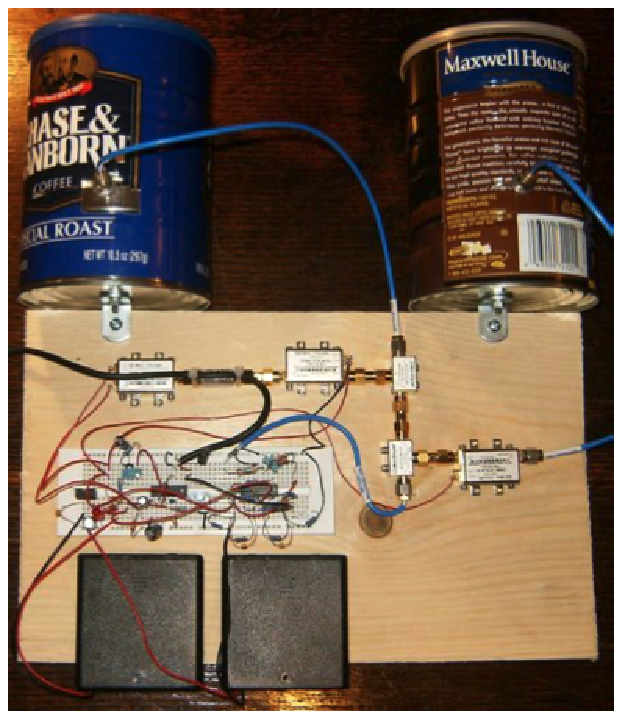
\includegraphics[width = 0.5\textwidth]{images/MITRadar.pdf}
    \caption{Completed MIT S-Band Radar}\label{MITRadar}\cite{charvat_mit_2012}
\end{figure}

The radar system is capable of measuring range, velocity and producing Synthetic Aperture Images. The project used the popular method of FMCW again because of the lower cost associated with the technology and the simple construction of the radar \cite{charvat_mit_2012}. The radar operates in the industrial, scientific and medical (ISM) band with $2.4 GHz$ being a common frequency. The transmitting power of the system is approximately $10 mW$ with a maximum range of 1km for $10 dBsm$. 

The radar makes use of two coffee cans as antennae where they both transmit and receive. The waveform generator generates a low power signal and is then amplified by the transmitter. The receiver passes the received signal through a filter where after the signal is amplified and fed into the analogue-to-digital (ADC) converter. After the signal is captured, the provided MATLAB code is used to process the data. 

The MIT radar opened up possibilities to students that were not previously possible. The whole radar was developed with reproducibility in mind. It is part of MIT's Open Courseware and the schematics, plans and instructions are completely open-source. The radar is also relatively low cost considering that radars for sea-going vessels can reach upwards of \$3000 \cite{noauthor_raymarine_nodate}. The sea-going vessels offer an easily accessible and tangible example of a working radar system. The MIT radar is also an accessible option where students can engage with how radar works and the processing behind it. Results obtained by a team attending the course at MIT can be seen in Figure \ref{MITResults}. The figure shows a Time vs Doppler plot with cars slowing down at a traffic light.
\begin{figure}[h!]
    \centering
    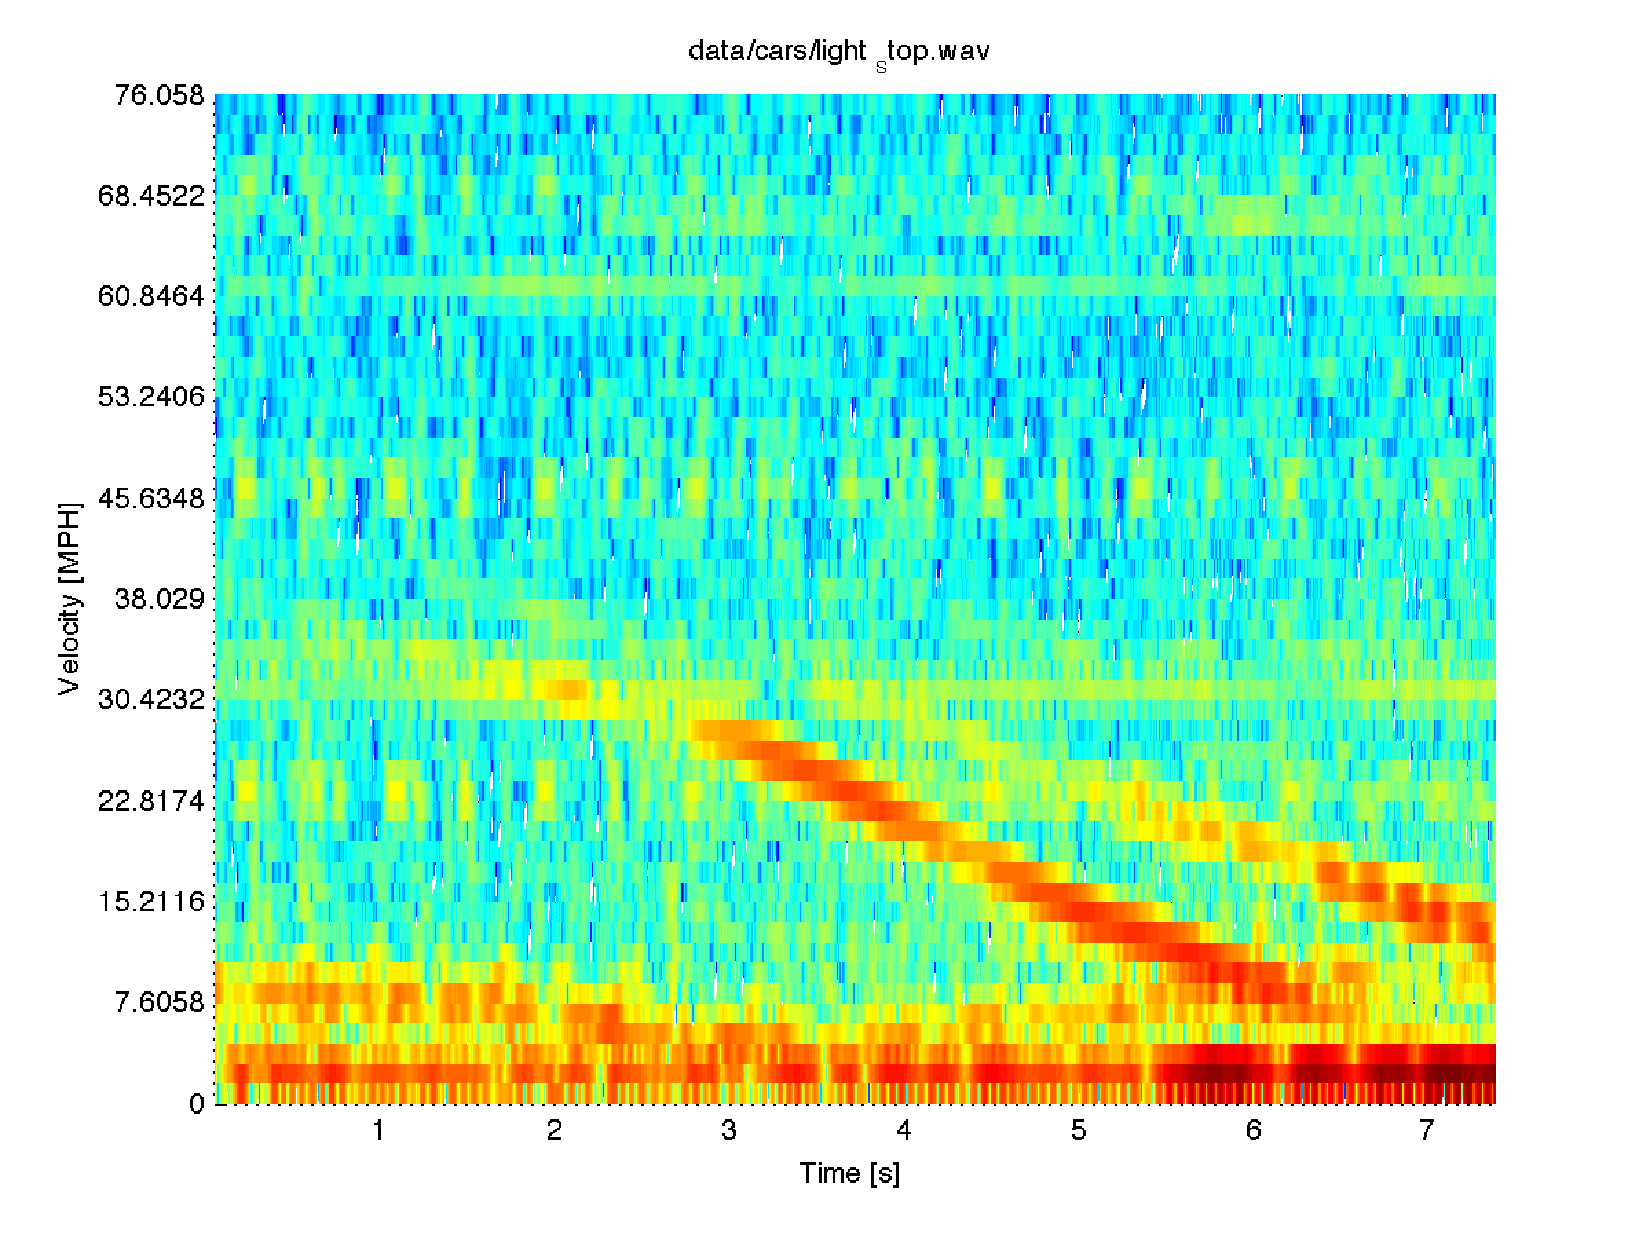
\includegraphics[width = 0.5\textwidth]{images/stop.pdf}
    \caption{MIT Radar Velocity Measurement \cite{charvat_mit_2012}}\label{MITResults}
\end{figure}

The radar system has a total cost of \$359.96 \cite{charvat_mit_2011} which makes the field of radar more accessible yet excludes the likes of high school students and university students without a formal course with funding. Apart from the cost involved with the radar, other drawbacks of the system are that it operates in the ISM band. This in itself is not a weakness but for an educational radar package, it would be beneficial to see or hear something tangible yield results. The physical size of the completed radar can also be viewed as a drawback since it is a cumbersome shape with two large coffee cans on its edge. The device is also prone to stop working with being dropped or knocked since RF components are rather sensitive.

\subsection{Other Educational Radar Programmes}
Several universities around the world offer undergraduate and postgraduate courses introducing the workings of radar systems. One such course is offered by the Johns Hopkins University's Whiting School for Engineering. The course covers everything needed to get a solid fundamental understanding of radars including antennae, the range equation, matched filtering and pulse Doppler to name a few. 

However, the course is offered at a prestigious university and attending a single course is not possible. The course also has prerequisites that prior knowledge of stochastic processes, MATLAB, DSP and electromagnetism making the course exclusive. There is also no practical aspect of the course \cite{noauthor_525.648introduction_nodate}.

Other universities do offer a single semester course in radar systems such as the University College London. The course is a four-day short-course focusing on the principles of modern radar systems and the signal processing associated with it. The course is for graduate-level engineers and a background in electronics and physics is required. It is possible to sign-up for this course as a standalone course or towards a masters level qualification.

The drawbacks of this course are once again that no practical and tangible results are obtained. The cost of the course is also expensive at \pounds1500 for four days. This course is not aimed at a high school or university students to spark interest in the radar research field. 

\section{Student-Developed Radar Systems}

The University of Cape Town (UCT) has a research centre specialising in Radar Systems. The centre drives research in the field especially in final year projects for engineers. One such engineer is Chiao-Shing Lin who completed his project in 2018. His project investigated the design and implementation of an audio radar for hand gesture recognition. He used an STM32F4 microcontroller to sample the audio between $8Khz$ and $12KHz$. All of the components needed to build the radar was developed from the ground up. The signal processing took place on a PC using MATLAB \cite{lin_design_2018}. 

The project proved to be a success with results showing that using the audible range of frequencies are indeed possible to recognise hand gesture such as the \textit{come-here} movement with a finger or \textit{spraying-water} gesture. Figure \ref{fig:linResults} shows results where one hand moved toward the radar and another away from it.

\begin{figure}[h!]
    \centering
    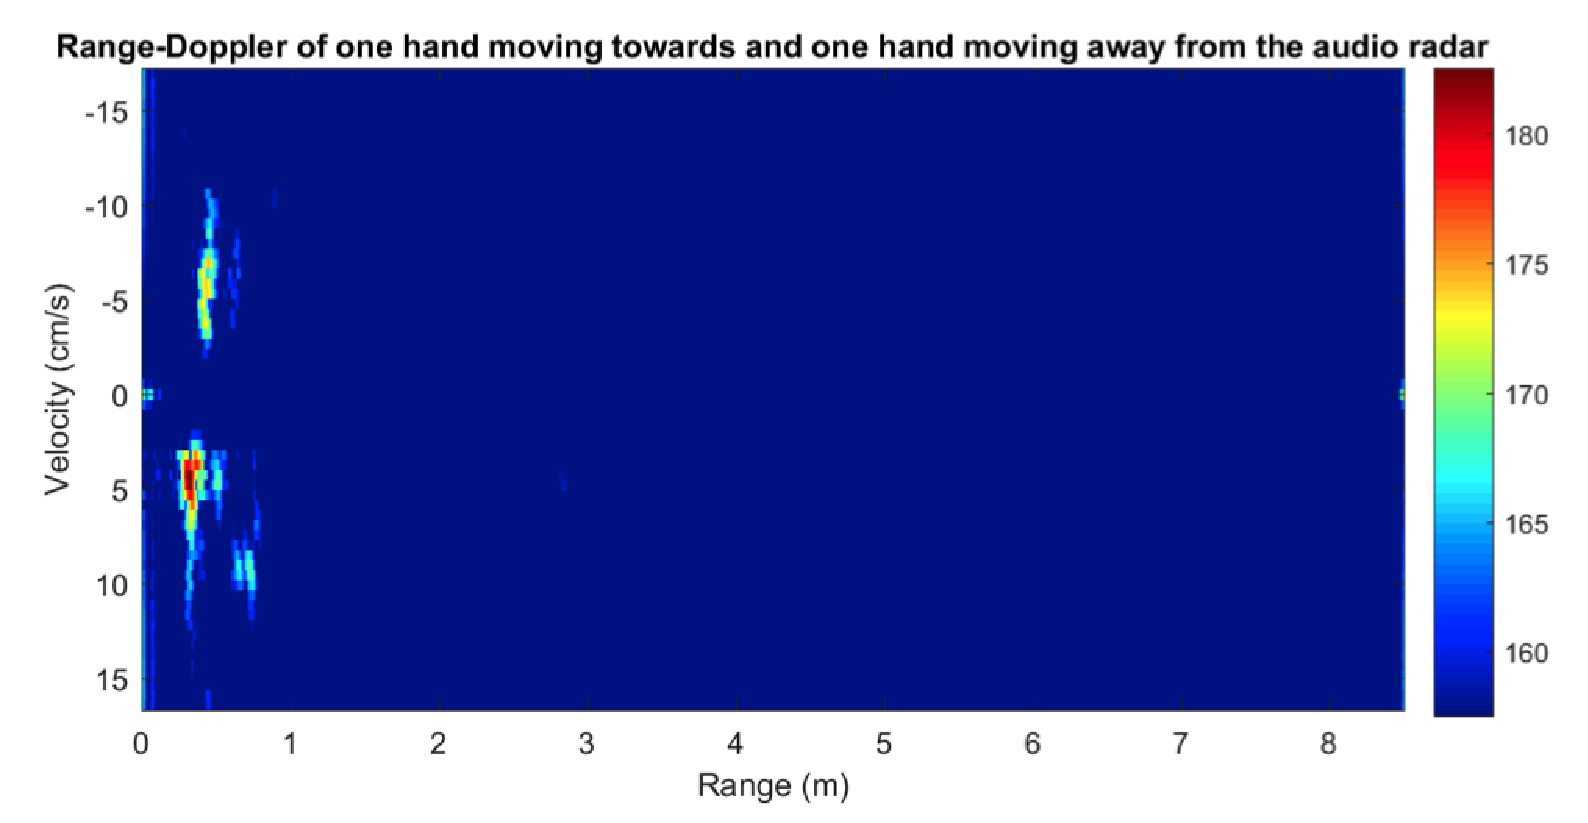
\includegraphics[width = 0.65\textwidth]{images/handmoving.pdf}
    \caption{Audible Radar Results}\label{fig:linResults}\cite{lin_design_2018}
\end{figure}

The project proved to be stricken for time as all of the components were built from scratch. It causes issues as prior advanced knowledge of circuitry should have been known to build the radar. The use of a computer to process the data is also essential, making the project too large for open days. The reproducibility of the project is low since the circuitry can be difficult to understand and build. 

A similar project at UCT for hand-gesture recognition was built by Rishad Ali Yasin. He focused on building a radar but in the ultrasonic sound spectrum. The radar was also built from the ground up but only using ultrasonic frequencies ($40KHz\ \pm\ 1KHz$) as the centre frequency. The signal processing also took place on a PC and the STM32F4 was also used in the project \cite{ali_yasin_design_2018}. Figure \ref{fig:ultrasonic} shows the physical implementation of the system.

\begin{figure}[h!]
    \centering
    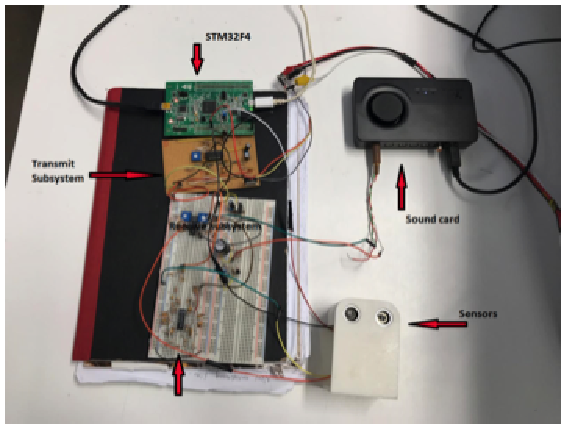
\includegraphics[width = 0.5\textwidth]{images/ultrasonic.pdf}
    \caption{Ultrasonic Implementation of Radar}\label{fig:ultrasonic}\cite{ali_yasin_design_2018}
\end{figure}

The project yielded successful results in recognising gestures such as moving towards and away from the transmitter/receiver with a corner reflector. Results from a test where hands and fingers were moving can be seen in Figure \ref{fig:aliresults}.
\begin{figure}[h!]
    \centering
    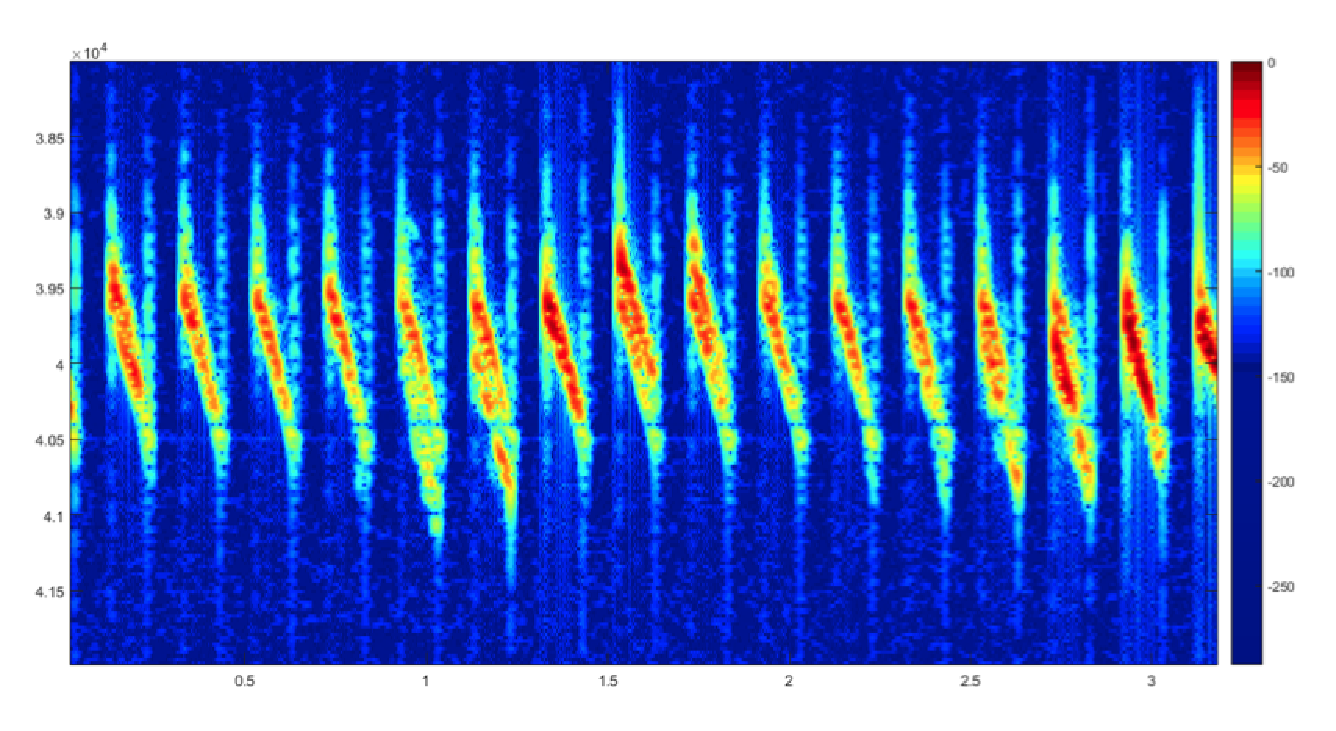
\includegraphics[width = 0.65\textwidth]{images/handsfingers.pdf}
    \caption{Ultrasonic Radar Results}\label{fig:aliresults}\cite{ali_yasin_design_2018}
\end{figure}

Both of the above-mentioned projects used the STM32F4 microcontrollers as an embedded platform but the need for the PC running MATLAB was still required to process the signals. This is a drawback in the context of presenting the data as well as the portability of the system.

\section{Commercial, Small-Scale Radar Systems}
Following the student developed radar systems, the commercial sector has some small-scale radar systems on offer for use in education and industry.
\subsection{uRad Radar System}
uRad is a Spanish start-up which is specifically focused on development small-scale embedded radar systems. They have developed a system that can be used as a \textit{Hardware-attached-on-top} (HAT) on a Raspberry Pi or as a module to attach to an Arduino Uno Revision 3. The option for a universal uRad radar also exists.

The system makes use of either FMCW in the form of a triangular wave as well as a sawtooth wave for modulating the transmitted signal. Both of these signals would be used to track the range of objects. The sawtooth modulated wave offers no velocity measurement but high accuracy in measurement of distance. The triangular modulated wave offers both velocity and distance measurement with high accuracy.

The uRad system also offers a Doppler CW mode that is used exclusively for radial velocity measurement and offers the best accuracy and very low complexity. The Arduino compatible uRad board can be seen in Figure \ref{uRadArduino} \cite{noauthor_urad_2018}.

\begin{figure}[h!]
    \centering
    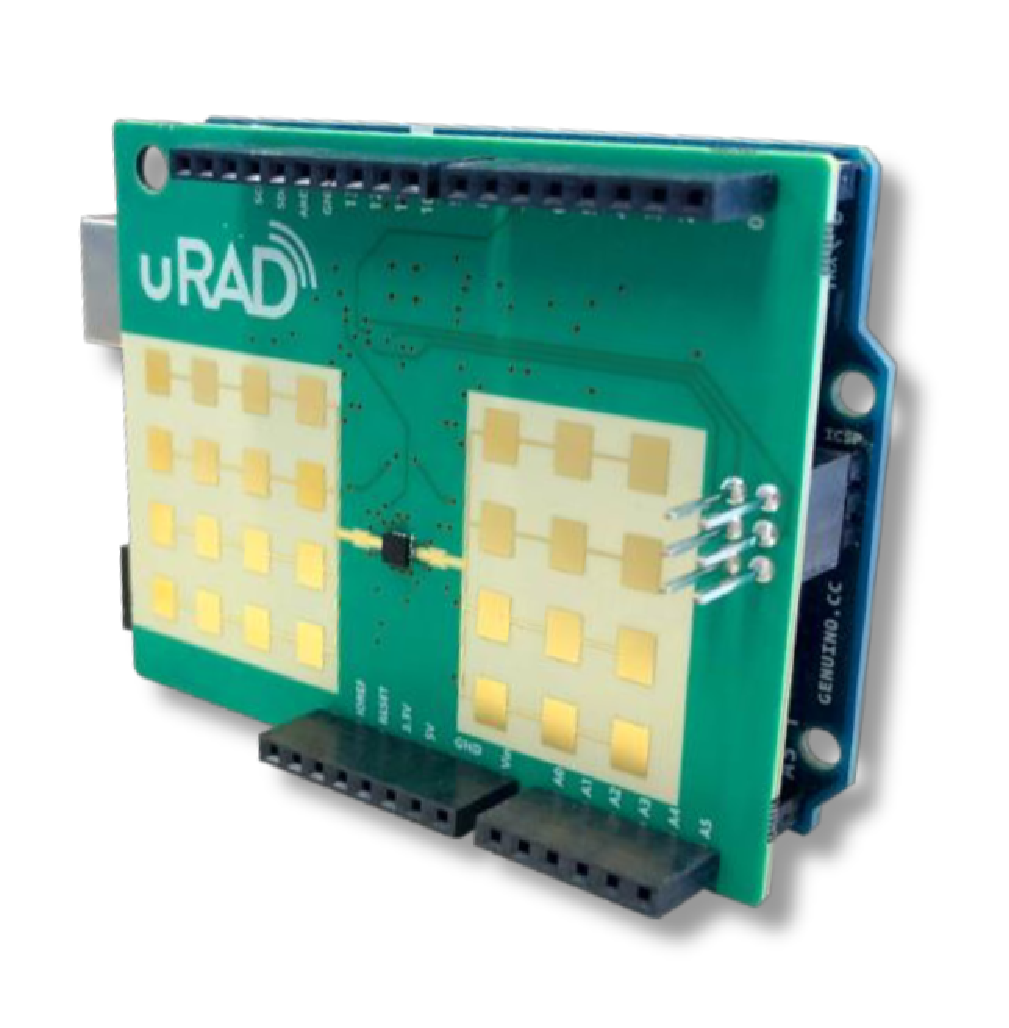
\includegraphics[width = 0.5\textwidth]{images/uRad.pdf}
    \caption{uRad Arduino compatible board \cite{noauthor_urad_2018-1}}\label{uRadArduino}
\end{figure}

The pulse repetition frequency (PRF) in the uRad system does not explicitly state but it can be considered to be fairly low given that the range of measurement is below $100\ m$. The uRad radar system operated within the noise-free ISM frequency band of $24\ GHz$ \cite{noauthor_microwave_2019}. The system operates with a minimum bandwidth of $24\ GHz$ and a maximum bandwidth of $24.25\ GHz$ giving the system bandwidth of $0.25\ GHz$. The targets used in the uRad radar system range from humans and birds to buildings and cars. It can detect objects within line of site but it is not a necessity. It can detect objects through walls as well. Therefore, it can be used as a security device to detect a presence within a building.

The uRad system is a very well packaged and accessible radar with a wide range of functionality ready for a commercial or \textit{tinkering} project. It also uses a generally available platform (Raspberry Pi and Arduino) which makes the option attractive. The radar yields very reliable results on a user friendly interface as can be seen in Figure \ref{uRadRes}. It is low-cost regarding radar equipment however, it excludes the generally interested parties of experimenting with radar systems since they are expensive to high school and university students. The system costs \euro$199$ for the add-on onto an existing Raspberry Pi or Arduino Uno.
\begin{figure}[h!]
    \centering
    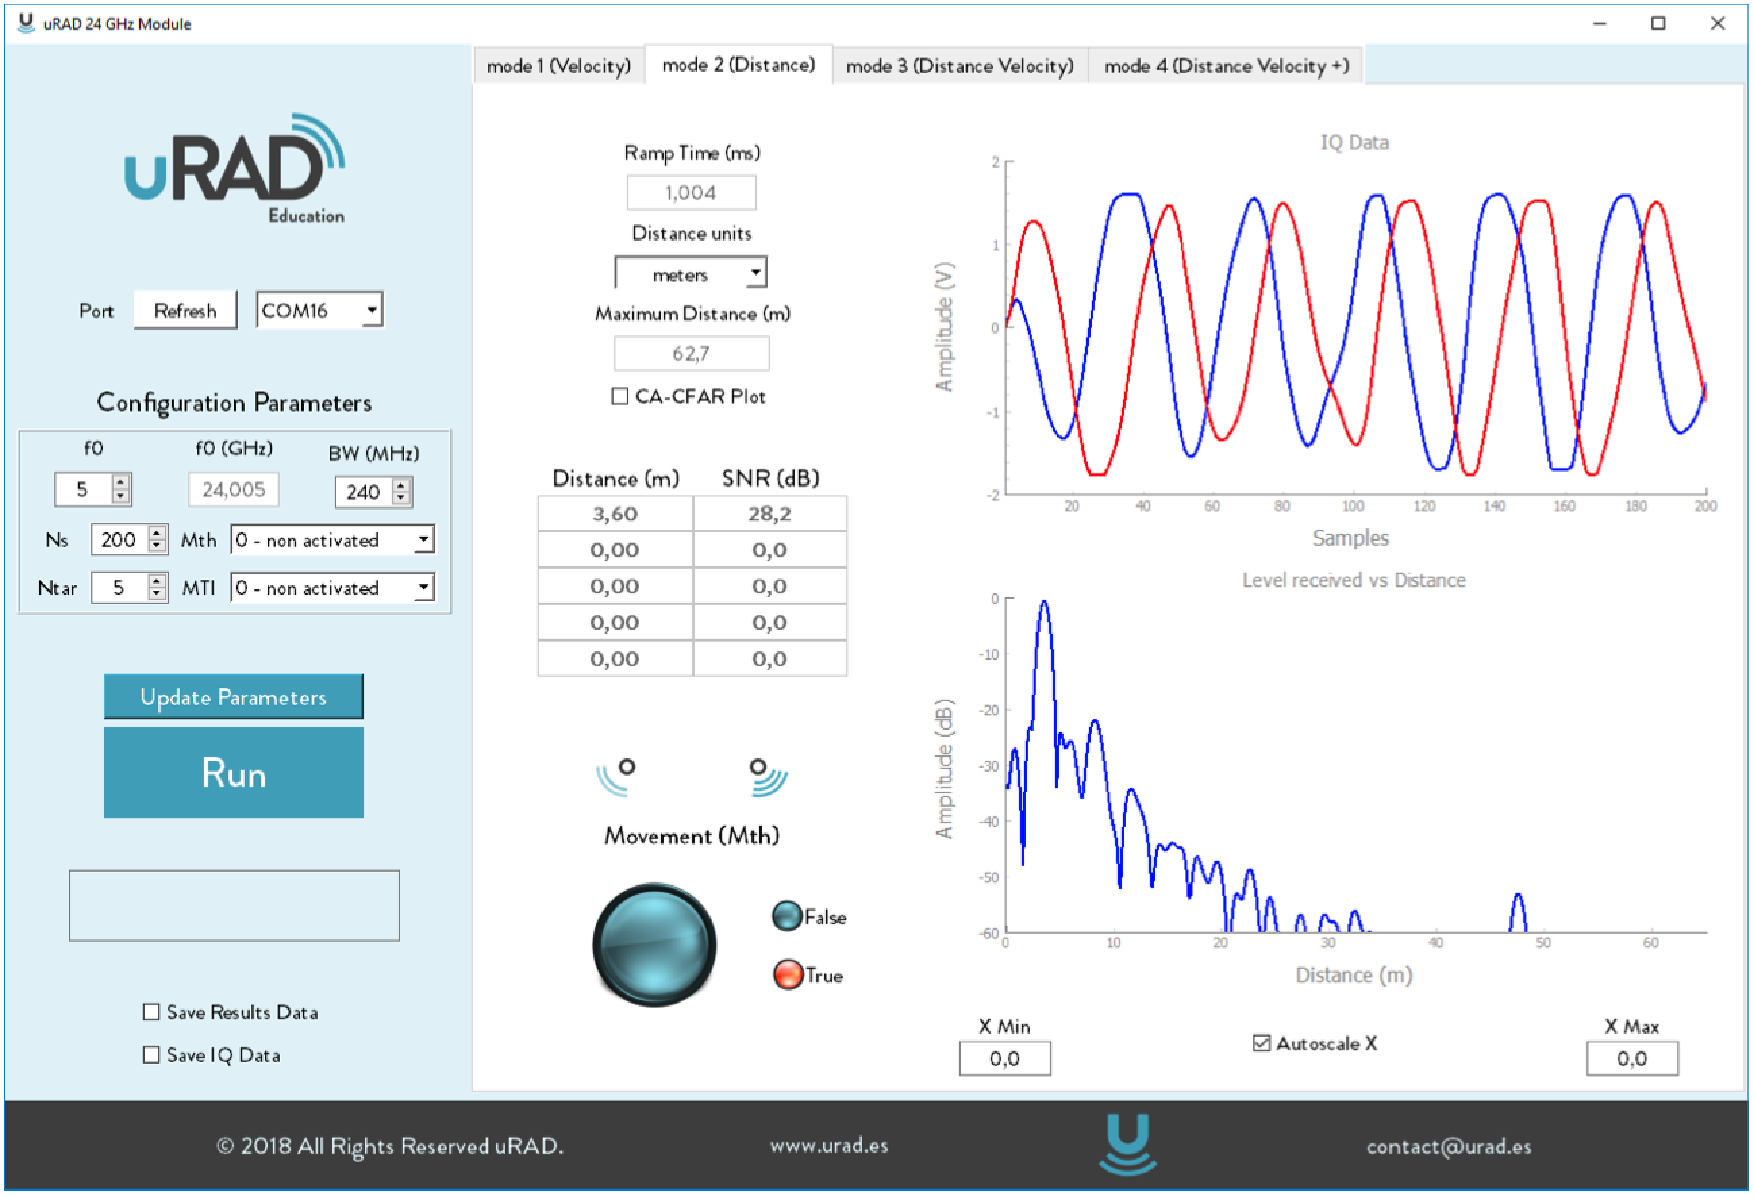
\includegraphics[width = 0.8\textwidth]{images/uRadRes.pdf}
    \caption{uRad Results \cite{noauthor_urad_2018-1}}\label{uRadRes}
\end{figure}

\subsection{Low-Cost Mini Radar}
Another research project is the monostatic radar developed by Tarchi et al. The Low-Cost Mini Radar uses FMCW and the reason for using FMCW was to keep the physical size of the package small. FMCW is a relatively old technology, hence it can be made into a relatively small footprint \cite{tarchi_low-cost_2017}. The small package is necessary since the project would be used on unmanned moving platforms. The Low-Cost Mini Radar uses a particularly high PRF of $26.2610\ MHz$. The high PRF offers acceptable range being relatively unambiguous at $100\ m$ but the high PRF also allows for accurate velocity measurement. The radar operates in the $K_u$ band with centre frequency $17.2\ GHz$. The bandwidth of the system is a maximum of $1.4\ GHz$. The Radar was used to detect parking signs, light poles, parked cars and an external staircase. A physical implementation of the radar system can be seen in Figure \ref{fig:LowcostminiRadar}.

\begin{figure}[h!]
    \centering
    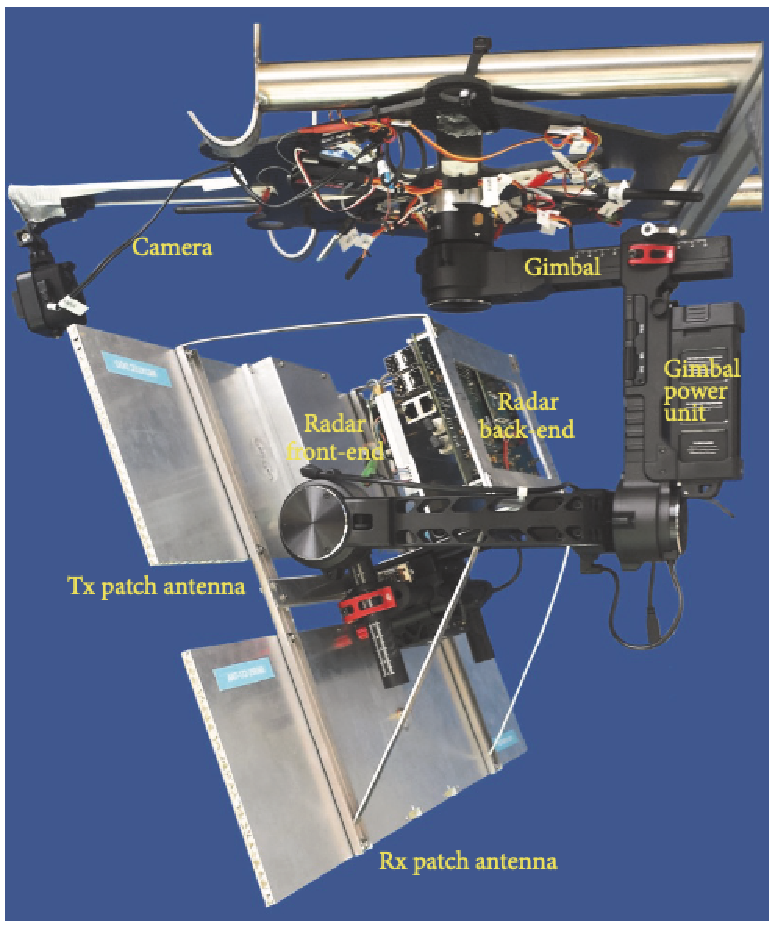
\includegraphics[width = 0.5\textwidth]{images/lowcostminiradar.pdf}
    \caption{Low-Cost Mini Radar for unmanned moving platforms \cite{tarchi_low-cost_2017}}\label{fig:LowcostminiRadar}
\end{figure}
Results obtained by the radar when tested in a parking lot (seen in Figure \ref{fig:LCtesting}) can be seen to identify parked cars, the tree line and a building wall in Figure \ref{fig:LCresults}.

\begin{figure}
    \centering
    \begin{minipage}{0.45\textwidth}
        \centering
        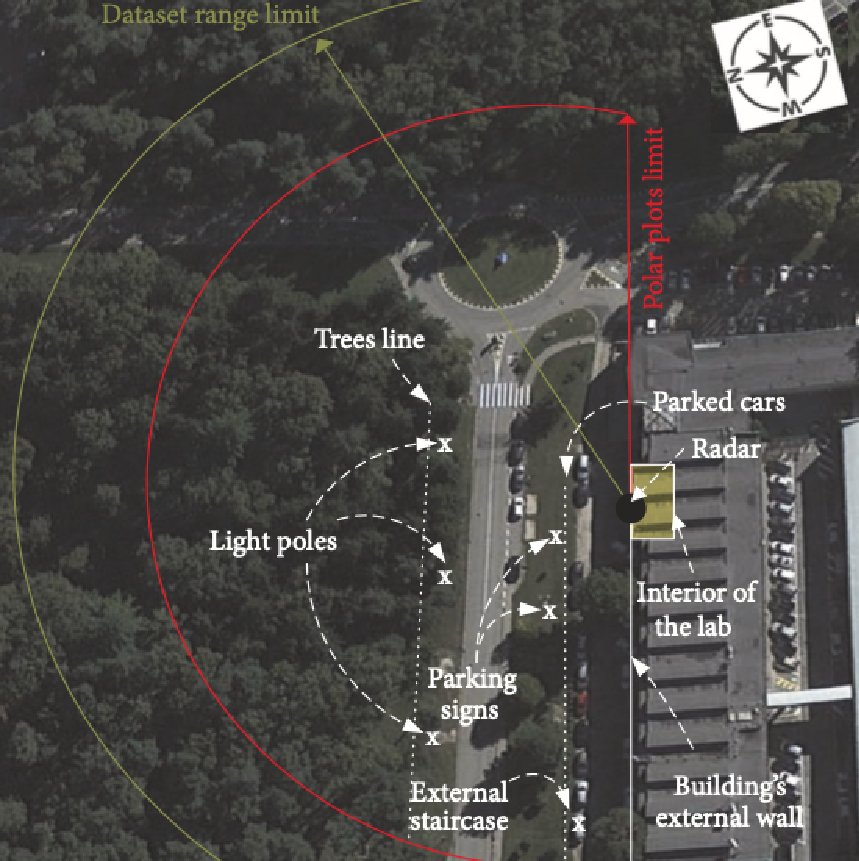
\includegraphics[width=0.9\textwidth]{images/tests.pdf}
        \caption{Testing ground for Low-Cost Mini Radar \cite{tarchi_low-cost_2017}}\label{fig:LCtesting}
    \end{minipage}\hfill
    \begin{minipage}{0.45\textwidth}
        \centering
        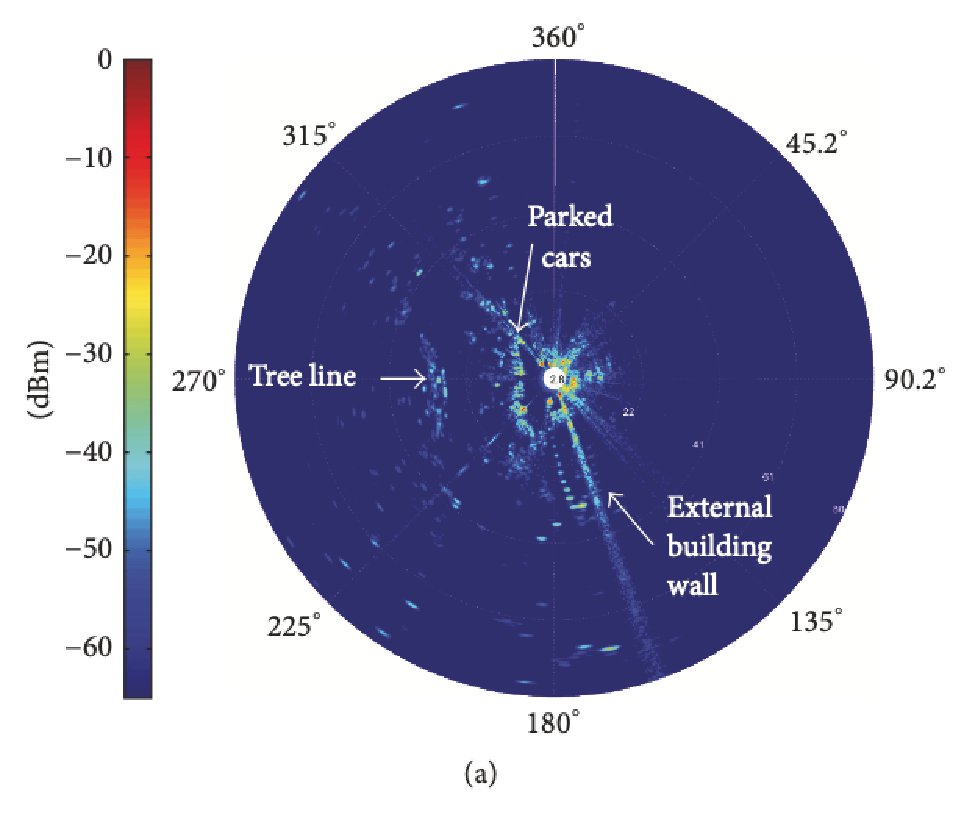
\includegraphics[width=0.9\textwidth]{images/lowcostradar.pdf}
        \caption{Results for Low-Cost Mini Radar \cite{tarchi_low-cost_2017}}\label{fig:LCresults}
    \end{minipage}
\end{figure}

\subsection{Conclusion}
In conclusion to the work laid out above, the Small-Scale, Embedded, Educational Audio Radar uses aspects from various previous works. The radar would need to implement a range and velocity measuring capabilities. Furthermore, the hardware and the implementation of radar systems are onerous and tend to be inaccessible to most. The radar systems investigated within this review are no different. The audio radar would improve on these short-comings in the following ways.

The MIT Radar offers an educational radar but still at a premium. The audio radar would reduce the cost and make radar technology even simpler without the need for expensive RF components. The accessibility of the designs and resources of the MIT radar would be utilised and mimicked in the audio radar to get more people involved in radar systems. The portability of the radar would be improved over the MIT radar but the simplicity of the radar would be maintained.

The educational courses offered worldwide attempt to provide an introduction to radar systems but the cost associated with it make them exclusive and difficult to attend given their physical location. The audio radar would attempt to make the data readily available and remove the barrier to the basic understanding of how these systems work.

Student developed radar systems form a vital part in the preparation and execution of this project. Previous research is used and refined upon in their work and would be done in this project as well. The processing of the signals in the student developed radars were all done after the data was collected and not in a timeous manner. The audio radar will process the data as soon as received to display results within seconds. The project would also make use of readily available \textit{breakout} boards to render the project even more accessible and usable as a learning tool.

The uRad offers a lot of similarities to the audio radar where it also detects the same objects at similar ranges. It offers up to $100\ m$ range, but the technology has the same focus. It is in a usable form factor using existing hardware\footnote{Raspberry Pi and Arduino}. The uRad system has a user friendly interface that the audio radar would build on. Most radar systems for low-cost implementation, including the uRad system, utilised the FMCW radar method since it is an older technology that is refined at this point but is more complex compared to CW. The audio radar would not implement FMCW but the theory behind it is still valuable to this project. The project would also improve on the portability of the radar and offering a PC free environment for obtaining results. This would be done using a web server linked to the back-end of the radar.

%It is important to note that the bandwidth in most of the systems above is roughly $\tfrac{1}{10}$\textsuperscript{th} the value of the centre frequency.

\newpage